\documentclass{article}
\usepackage[utf8]{inputenc}

\title{MATH3160 — Portfolio 4.2b}
\author{Mike Medved}
\date{October 8th, 2022}

\usepackage{color}
\usepackage{amsthm}
\usepackage{amssymb} 
\usepackage{amsmath}
\usepackage[margin=1in]{geometry} 
\usepackage{listings}
\usepackage[dvipsnames]{xcolor}
\usepackage{tikz}

\begin{document}

\maketitle

\section{Deliverables}

\subsection{Moment Generating Function (mgf)}

The moment generating function of a discrete random variable can be represented as $M_X(t) \to \left[0, \infty\right]$ where

$$
M_X(t) = E\left[e^{tX}\right]
$$

\subsubsection{Example of 1.1}

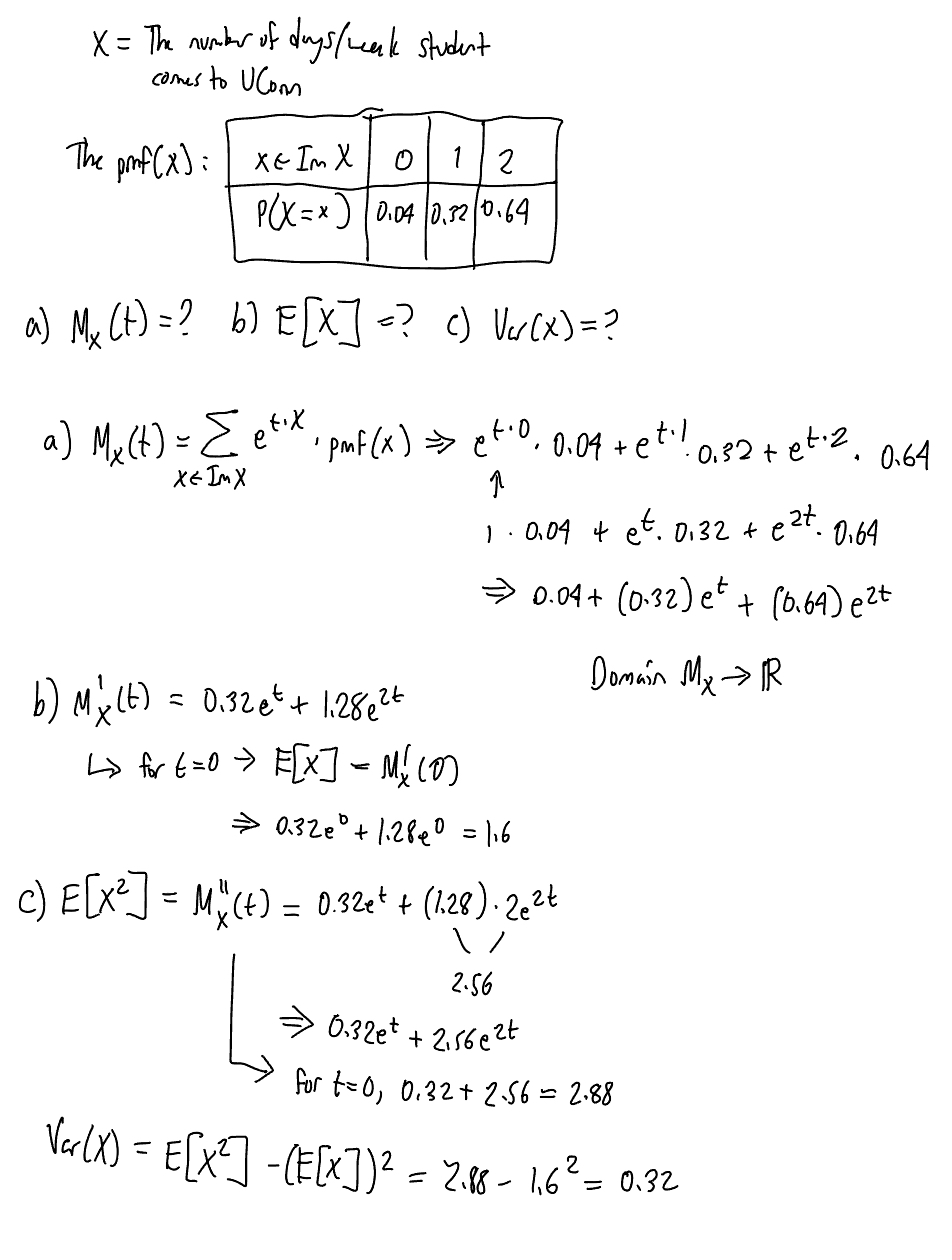
\includegraphics[height=5.5in]{example-mgf.jpeg}

\end{document}